% SPDX-License-Identifier: CC-BY-SA-4.0
%
% Copyright (C) 2026 embedded brains GmbH & Co. KG
\documentclass[tikz,border=4pt]{standalone}
\usepackage[T1]{fontenc}
\usepackage[scaled]{helvet}
\renewcommand{\familydefault}{\sfdefault}
\usetikzlibrary{arrows.meta,backgrounds,positioning,calc}
\definecolor{ebblue}{HTML}{1F4E79}
\definecolor{boxfill}{HTML}{EAF1F8}
\definecolor{groupfill}{HTML}{F5F5F5}
\definecolor{codeline}{HTML}{9C6500}
\definecolor{flow}{HTML}{404040}
\begin{document}
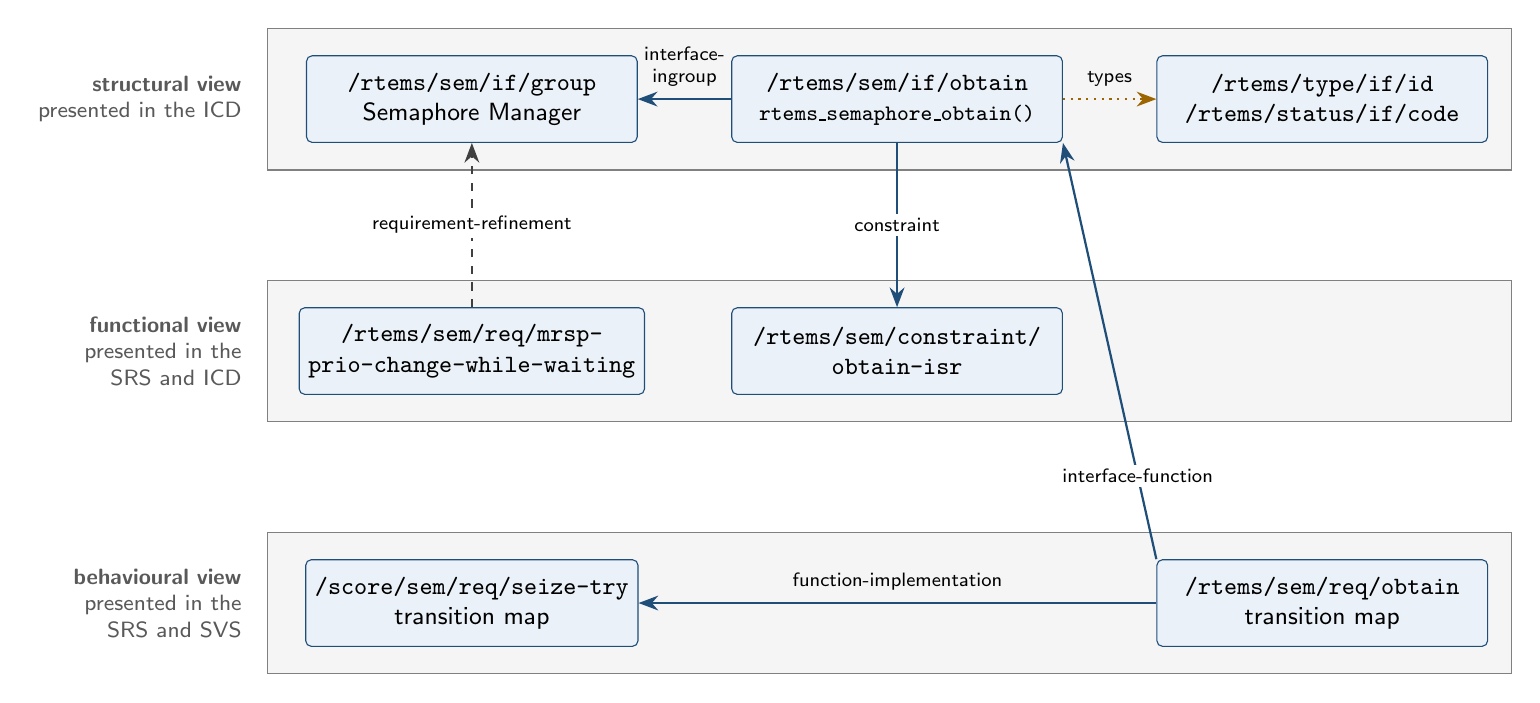
\begin{tikzpicture}[
    font=\small,
    item/.style={draw=ebblue, fill=boxfill, rounded corners=2pt,
      minimum width=42mm, minimum height=11mm, align=center},
    lanelabel/.style={font=\footnotesize, text=gray!70!black,
      align=right, anchor=east, text width=26mm},
    link/.style={-{Stealth[length=2.5mm]}, thick, draw=ebblue},
    refine/.style={-{Stealth[length=2.5mm]}, thick, dashed, draw=flow},
    names/.style={-{Stealth[length=2.5mm]}, thick, dotted, draw=codeline},
    lbl/.style={font=\scriptsize, fill=groupfill, inner sep=1.5pt,
      align=center}]

  \def\xa{2.4}\def\xb{7.8}\def\xc{13.2}
  \def\left{-0.2}\def\right{15.6}
  \foreach \y/\name/\doc in {5.8/structural view/ICD,
      2.6/functional view/SRS and ICD,
      -0.6/behavioural view/SRS and SVS} {
    \fill[groupfill] (\left,\y-0.9) rectangle (\right,\y+0.9);
    \draw[gray] (\left,\y-0.9) rectangle (\right,\y+0.9);
    \node[lanelabel] at (\left-0.2,\y)
      {\textbf{\name}\\presented in the \doc};
  }

  \node[item] (semgroup) at (\xa,5.8)
    {\texttt{/rtems/sem/if/group}\\Semaphore Manager};
  \node[item] (obtainif) at (\xb,5.8)
    {\texttt{/rtems/sem/if/obtain}\\
     \footnotesize\texttt{rtems\_semaphore\_obtain()}};
  \node[item] (types) at (\xc,5.8)
    {\texttt{/rtems/type/if/id}\\\texttt{/rtems/status/if/code}};

  \node[item] (mrsp) at (\xa,2.6)
    {\texttt{/rtems/sem/req/mrsp-}\\
     \texttt{prio-change-while-waiting}};
  \node[item] (isr) at (\xb,2.6)
    {\texttt{/rtems/sem/constraint/}\\\texttt{obtain-isr}};

  \node[item] (seize) at (\xa,-0.6)
    {\texttt{/score/sem/req/seize-try}\\transition map};
  \node[item] (obtainreq) at (\xc,-0.6)
    {\texttt{/rtems/sem/req/obtain}\\transition map};

  \draw[link] (obtainif) -- node[lbl, above=1mm, fill=none]
    {interface-\\ingroup} (semgroup);
  \draw[names] (obtainif) -- node[lbl, above=1mm, fill=none]
    {types} (types);
  \draw[refine] (mrsp) -- node[lbl, fill=white]
    {requirement-refinement} (semgroup);
  \draw[link] (obtainif) -- node[lbl, fill=white] {constraint} (isr);
  \draw[link] (obtainreq.north west) -- node[lbl, pos=0.2, fill=white]
    {interface-function} (obtainif.south east);
  \draw[link] (obtainreq) -- node[lbl, above=1mm, fill=none]
    {function-implementation} (seize);
\end{tikzpicture}
\end{document}
